\subsection{Standard Model W+Jets}
\label{sec:Bkg:wjet}

\indent A $W$ boson produced in conjunction with QCD jets ($W$+jets) is our largest subdominant background.  $W$+jets comprises 9 percent of the total background in the signal region.  However the distribution of $W$+jets is not uniform across $\RISR$.  $W$+jets can reach 20-25 percent of all backgrounds in signal region bins with the largest $\RISR$.  This means the $W$+jets contribution mostly affects high stop mass samples because those signal samples peak at high $\RISR$. \\

\indent We estimate $W$+jets using an one lepton control region defined in table \ref{tab:WJetCR}..  The one lepton $W$+jet control region is designed to ensure high $W$+jet purity.   All one lepton control regions are mutually exclusive including the ttbar, $W$+jets and single top control region. \\

\begin{table}[h!]
  \begin{center}
    \begin{tabular}{c||c}
      \hline \hline
          {\bf Variables }                           & $W$+jets control region                \\ \hline \hline
      Number of leptons             & 1                                          \\ 
      Number of jets (incl. lepton) & $\geq 4$                                     \\ 
      $\pt$ of jets (incl. lepton)  & (80,80,40,40) GeV                            \\ 
      \mindphijettwomet             & $> 0.4$                                      \\ 
      $\met$                        & $>250$ GeV                                   \\ 
      \mtlepmet                     & ($>30, <100$ GeV) \\ 
      Number of $b$-jets            & $=1$                            \\ 
      \mantikttwelvezero            & $<60\,$GeV         \\ 
      \mindrblep                    & $>2.0$             \\ \hline \hline
    \end{tabular}
  \end{center}
  \caption{Summary of the selection for the one lepton $W$+jets control region.}
  \label{tab:WJetCR}
\end{table}

\indent The lepton is treated as a jet for the jet multiplicity and the jet $\pt$ requirements.  Similar to the one lepton $\ttbar$ control region, the lepton is meant to play the role of a hadronic tau jet in the zero-lepton signal region.  \\

\indent $\mtlepmet$ is defined in equation \ref{eqn:mtlep} as the transverse mass of the lepton and the $\met$.  The $\mtlepmet$ selection ensures that the transverse mass is consistent with those originating from a $W$ boson.  \\

\indent Orthogonality between the $W$+jet control region and the single top control region is ensured by the requirement on the number of $b$-jets.  Orthogonality between $\ttbar$ control region and $W$+jet control region is ensured by the selection on $\mindrblep$.  $\mindrblep$ is defined in equation \ref{eqn:mindrblep} as the minimum $\Delta R$ between the two jets with the highest b-tag value and the selected lepton. \\

\indent $\mantikttwelvezero$ is defined as the mass of an $\antikt$ jet built with a distance parameter of $R=1.2$ instead of regular $R=0.4$.  The $\antikt$ algorithm clusters calorimeter energy into a jet according to the distance metric $R$ and is covered in detail in section \ref{sec:jet:reco}.  The $\antikt$ algorithm will form a perfectly conical jet of radius $R$ if no other hard objects are found within a cone of $2R$.  If two hard objects exist within $R<\Delta R<2R$ of one another then two jets will be formed splitting the energy cells between them.  \\

\indent The large R=1.2 jet is designed to cluster all the energy of a boosted top quark into a single jet.  If the jet contains a boosted top, the invariant mass of jet should be close to $\sim m_t$. The $\mantikttwelvezero < 60 \gev$ is designed to reject events with reconstructed boosted tops.  \\

\indent  Distributions of select kinematic variables in the $\Wjets$ control region are shown in Figure ~\ref{fig:CRWpts}.  The MC background has been normalized to data by performing a simultaneous fit to all control regions.  The hashed bands on the total SM background correspond to the total experimental systematical uncertainty plus the MC statistical uncertainty.  The yield in the $\Wjets$ control region is given in Table~\ref{table.bkgonly.CRW}.  \\

\indent  The fitted $W$+jets normalization scale factor is $1.27 \pm 0.15$.  Data and MC are compatible to within statistical uncertainty.  No strong trends are observed in the data to MC ratios in any of the distributions. \\

\begin{figure}[!h]
  \centering
  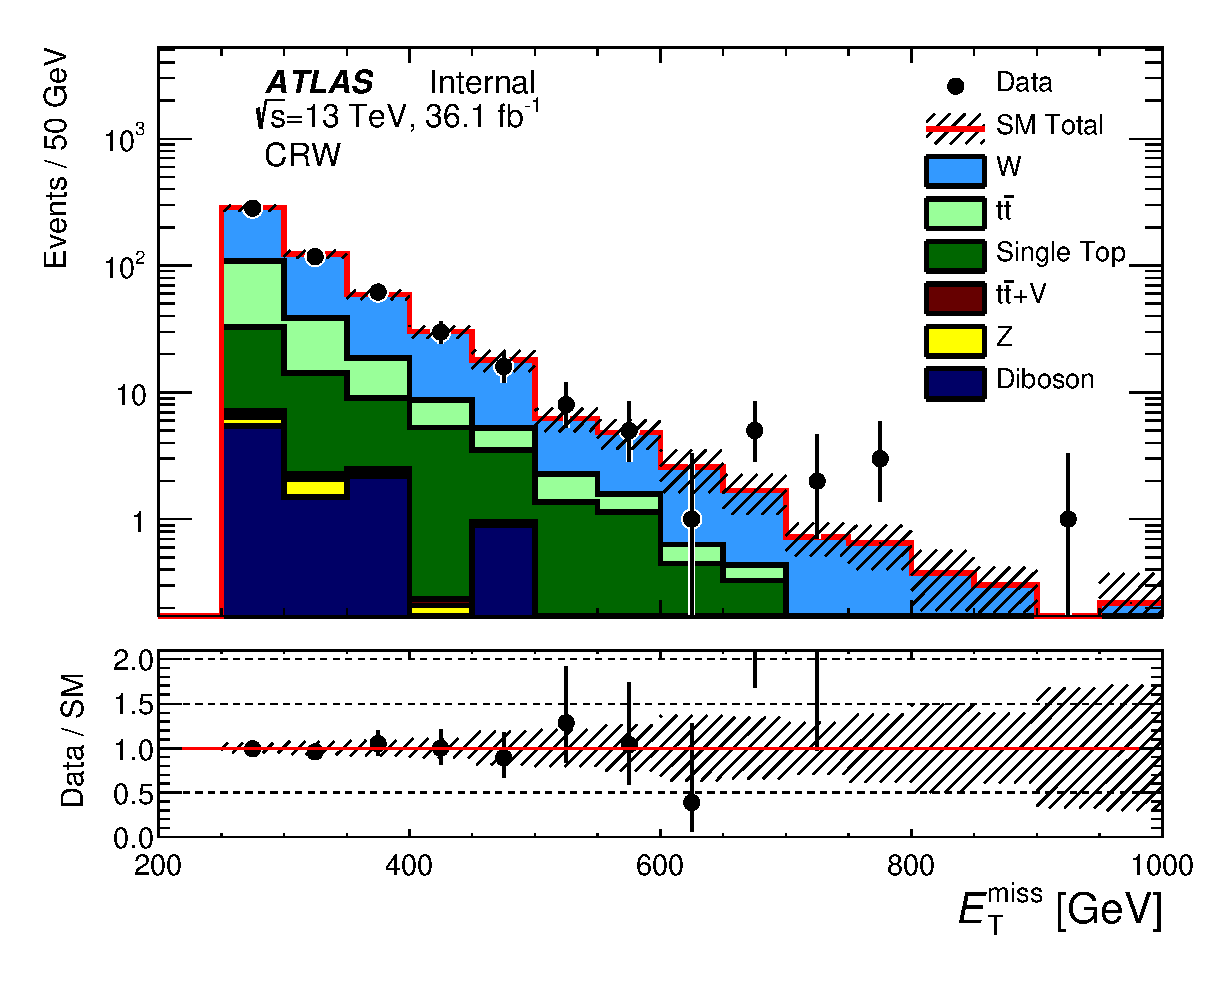
\includegraphics[width=0.45\textwidth]{figures/wJets/postfit/Met_CRW_log.eps}
    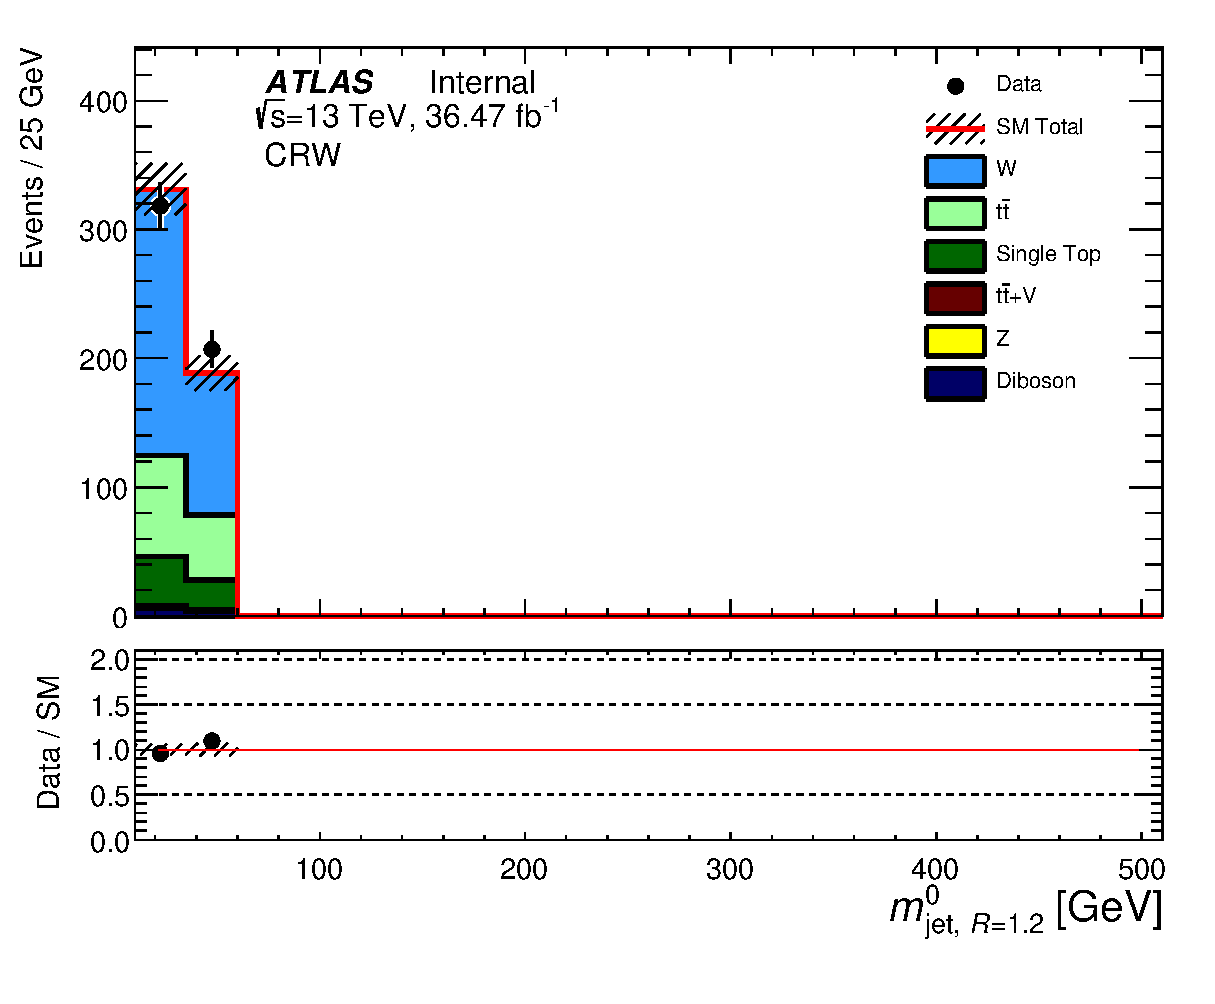
\includegraphics[width=0.45\textwidth]{figures/wJets/postfit/AntiKt12M_0__CRW.eps}
  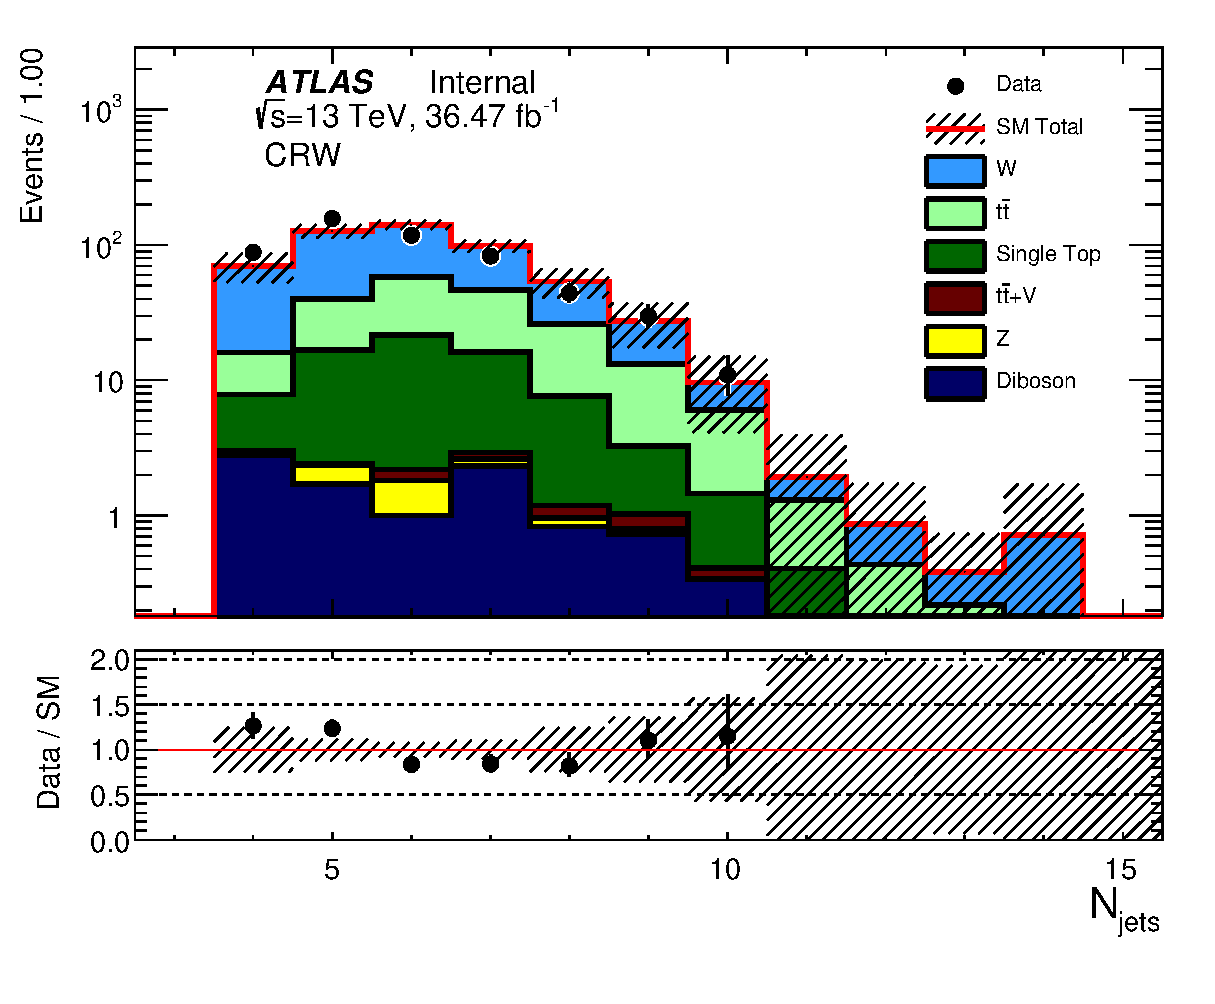
\includegraphics[width=0.45\textwidth]{figures/wJets/postfit/NJets_CRW_log.eps}
  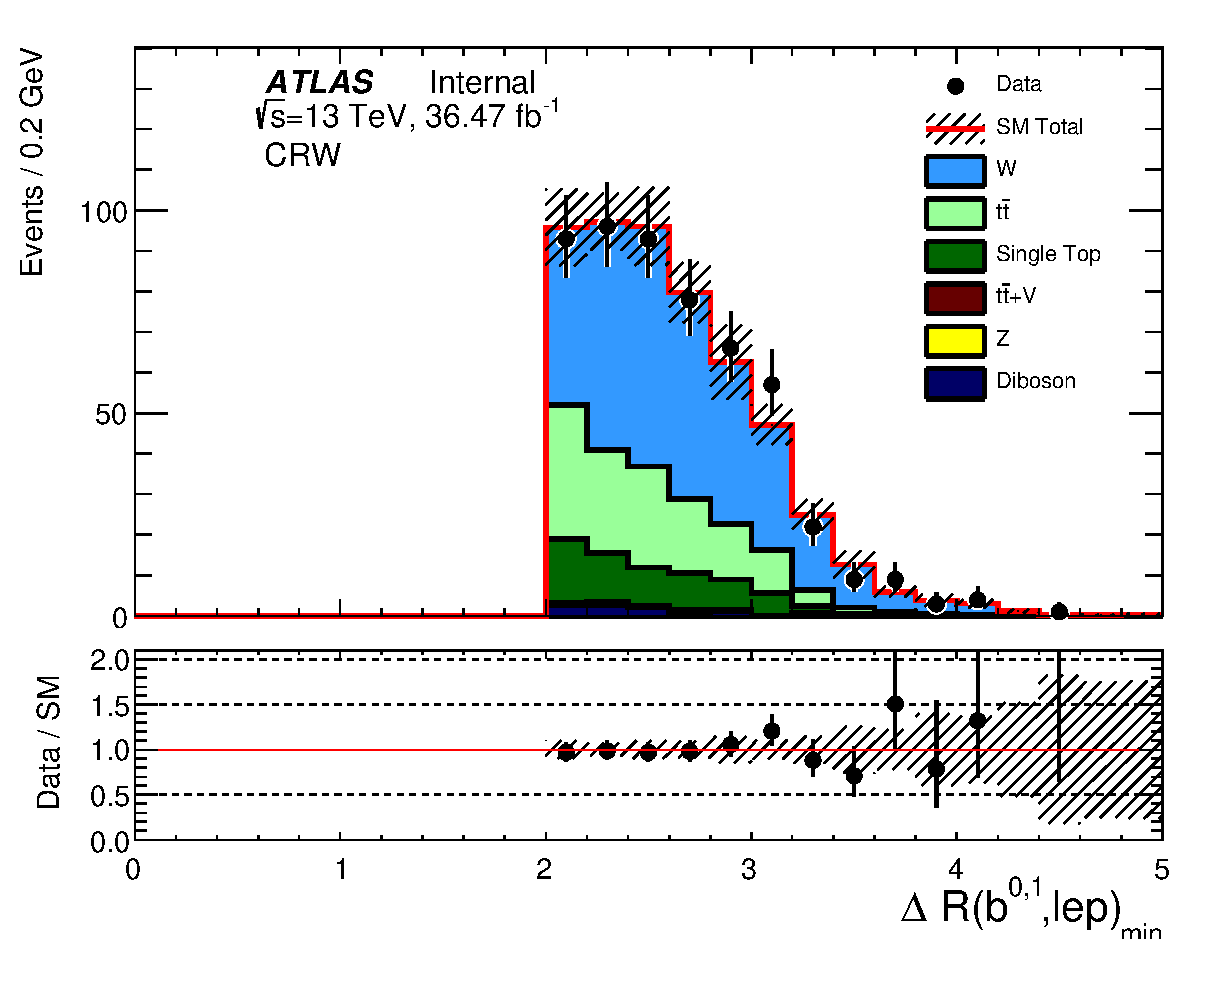
\includegraphics[width=0.45\textwidth]{figures/wJets/postfit/MinDRBLep_CRW.eps}]
  \caption[Kinematic distributions in the $\Wjets$ control region after the background only fit to $\intlumi$ $\ifb$ of data]{Kinematic distributions in the $\Wjets$ control region after the background only fit to $\intlumi$ $\ifb$ of data. From left to right and top to bottom, the variables shown are $\met$, $\mtlepmet$, $\mantikttwelvezero$ and the number of jets and $\mindrblep$. The expected SM background has been normalized to the data by performing a simultaneous fit to all control regions.  The hatched band on the total SM background correspond to the total experimental systematic uncertainty plus the MC statistical uncertainty.}
  \label{fig:CRWpts}
\end{figure}



\begin{table}[h!]
\caption[$W$+jets control region MC Yield and background-only fit results for $\intlumi$ $\ifb$ of data]{$W$+jets control region MC Yield and background-only fit results for $\intlumi$ $\ifb$ of data. MC exp. events are expected background rates directly from MC predictions.  Fitted background event rates are the expected background rates after normalizing the MC to data by simultaneously fitting all control regions using a background only fit.  The fitted $W$+jets normalization scale factor is equal to (Fitted $\Wjets$ events)/(MC exp. $\Wjets$ events). The quoted uncertainties include statistical and systematic uncertainties. }
\label{table.bkgonly.CRW}
\begin{center}
\setlength{\tabcolsep}{0.0pc}
{\small
%%
\begin{tabular*}{\textwidth}{@{\extracolsep{\fill}}lr}
\noalign{\smallskip}\hline\noalign{\smallskip}
{\bf CRW yields}           & CRW                      \\[-0.05cm]
\noalign{\smallskip}\hline\noalign{\smallskip}
%%
Observed events          & $533$                       \\
\noalign{\smallskip}\hline\noalign{\smallskip}
%%
Fitted bkg events         & $533.23 \pm 23.09$                 \\
\noalign{\smallskip}\hline\noalign{\smallskip}
%%
        Fitted TTbar events         & $115.60 \pm 18.76$                     \\
%%
        Fitted Wjets events         & $349.54 \pm 38.87$                  \\
%%
        Fitted Zjets events         & $1.86 \pm 0.63$                   \\
%%
        Fitted TtbarV events         & $1.15 \pm 0.43$                     \\
%%
        Fitted SingleTop events         & $54.76 \pm 20.41$                     \\
%%
        Fitted Diboson events         & $10.31 \pm 2.34$                    \\
%%
        Fitted Multijets events         & $0.00 \pm 0.00$                 \\
%%     
 \noalign{\smallskip}\hline\noalign{\smallskip}
%%
MC exp. SM events              & $458.28 \pm 21.31$                     \\
\noalign{\smallskip}\hline\noalign{\smallskip}
%%
        MC exp. TTbar events         & $122.28 \pm 15.29$                   \\
%%
        MC exp. Wjets events         & $276.00 \pm 5.53$             \\
%%
        MC exp. Zjets events         & $1.79 \pm 0.52$                     \\
%%
        MC exp. TtbarV events         & $0.89 \pm 0.35$                      \\
%%
        MC exp. SingleTop events         & $47.00 \pm 5.70$                   \\
%%
        MC exp. Diboson events         & $10.31 \pm 2.35$                   \\
%%
        MC exp. Multijets events         & $0.00 \pm 0.00$                \\
%%     \\
\noalign{\smallskip}\hline\noalign{\smallskip}
Fitted $W$+jets normalization scale factor & $1.27 \pm 0.15$ \\
\noalign{\smallskip}\hline\noalign{\smallskip}
\end{tabular*}
%%%
}
\end{center}
\end{table}
%

%\begin{table}[!h]
%  \centering
%  \begin{tabular}{c|c}
\hline\hline
\multicolumn{2}{c}{\bf CRW (60\% purity)} \\ \hline 
Z & 1.99 $\pm$ 0.45 \\
dibosons & 9.85 $\pm$ 1.76 \\
ttbar & 128.42 $\pm$ 3.82 \\
singleTop & 51.14 $\pm$ 3.37 \\
ttV & 1.07 $\pm$ 0.16 \\
W & 288.12 $\pm$ 8.86 \\
\hline
Total MC & 480.58 $\pm$ 10.38 \\
Data & 531.00 $\pm$ 23.04 \\
 \hline
SF & 1.17 $\pm$ 0.10 \\
\hline\hline
\end{tabular}

%  \caption{Yields in the $\Wjets$ CR with \intlumi\ \ifb\ of data.  }
%  \label{tab:CRW_yields}
%\end{table}

